\chapter{DESAIN}
\label{chapter:design}
Pada bab ini akan dijelaskan mengenai desain algoritma yang digunakan untuk menyelesaikan permasalahan pada Tugas Akhir ini.
\section{Desain Umum Sistem}	
Sistem pertama kali akan menjalankan fungsi MAIN terlebih dahulu. Desain dari fungsi MAIN dapat dilihat pada Gambar \ref{fig:mainfx}. %Masukan fungsi ini diperoleh dari studi kasus, sedangkan keluaran dari fungsi ini tidak ada. Proses yang dilakukan pada fungsi ini adalah:
%\begin{enumerate}
%\item menerima masukan berupa kasus uji coba, batas atas panjang kunci, \plaintext dan \textit{ciphertext}.
%\item Menjalankan fungsi SOLVE.
%\end{enumerate}
	
	  \begin{table}[H]
	 	\caption{Masukan, Proses, dan Keluaran fungsi MAIN}
		%\resizebox{\textwidth}{!}
		\label{tab:iomain}
	\end{table}

\begin{figure}[H]
		\centering
		
		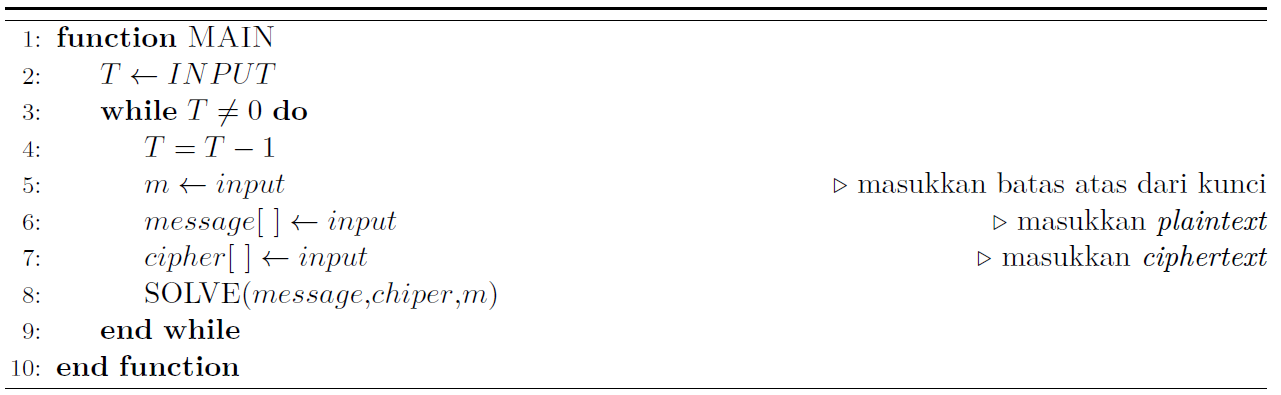
\includegraphics[scale=0.31]{images/bab3/mainfx.png}
		\caption{Gambar Fungsi Main}
		\label{fig:mainfx}
	\end{figure}
	
\begin{table}[H]
	 	\caption{Penjelasan variabel yang digunakan dalam fungsi MAIN}
		%\resizebox{\textwidth}{!}
		\label{tab:mainvar}
	\end{table}
	
\section{Desain Algoritma}
 Pada bagian ini akan dibahas secara rinci mengenai fungsi-fungsi yang digunakan dalam sistem.  
  \subsection{Desain fungsi SOLVE}
  \label{chapter:fxsolve}
  Fungsi ini digunakan untuk menyelesaikan permasalahan yang diangkat pada tugas akhir ini. Tahapan-tahapan prosesnya terdapat pada subbab \ref{chapter:dasar-teori} dan subbab \ref{chapter:solving}. Pada bagian ini tidak dapat mengecek kebenaran dari suatu panjang kunci. Gambar mengenai fungsi SOLVE dapat dilihat pada Gambar \ref{fig:solvefx1} dan \ref{fig:solvefx2}. %Masukan fungsi ini adalah \textit{plaintext}, \textit{ciphertext}, dan batas atas panjang kunci yang diperoleh dari fungsi MAIN. Keluaran dari fungsi ini adalah \plaintext yang telah direkonstruksi ulang. Proses yang terjadi pada fungsi ini yaitu
  %\begin{enumerate}
  %\item Mencari semua posisi, jumlah dimana \plaintext dan \ciphertext tidak bernilai '*'.
  %\item Mencari semua posisi dimana \ciphertext tidak bernilai '*' dan \plaintext bernilai '*'.
  %\item Mengiterasi panjang kunci dari $\frac{m}{2}+1$ sampai dengan $m$.
  %\item Melakukan \textit{intersection}. Cara yang digunakan untuk melakukan \textit{intersection} dapat dilihat di subbab \ref{chapter:solving} pada point yang terakhir.
%  \end{enumerate}
  
  \begin{table}[H]
	 	\caption{Masukan, Proses, dan Keluaran fungsi SOLVE}
		%\resizebox{\textwidth}{!}{%
		\begin{tabular}   {|p{2cm}|p{4.5cm}|p{2.5cm}|}\hline
		Masukan&Proses&Keluaran \\ \hline
		\textit{Plaintext}, \textit{ciphertext}, dan batas atas panjang kunci yang diperoleh dari fungsi MAIN&Mencari semua posisi, jumlah di mana \plaintext dan \ciphertext tidak bernilai "*". Mencari semua posisi di mana \ciphertext tidak bernilai "*" dan \plaintext bernilai "*". Mengiterasi panjang kunci dari $\frac{m}{2}+1$ sampai dengan $m$. Melakukan \textit{intersection}.  &\textit{Plaintext} yang telah direkonstruksi ulang \\ \hline
		\end{tabular}%}
		\label{tab:iosolve}
	\end{table}

	Mengenai modulo 26 yang terdapat pada Gambar \ref{fig:solvefx1} dan Gambar \ref{fig:solvefx2} digunakan untuk memastikan bahwa selisih dari \plaintext dan \ciphertext adalah pasti $< 26$. Ditambah 26 pada Gambar \ref{fig:solvefx1} dan Gambar \ref{fig:solvefx2} dimaksudkan agar silisih antara \plaintext dan \ciphertext selalu bernilai positif.  
  
  
  \begin{figure}[H]
		\centering
		%\resizebox{\textwidth}{!}{%
		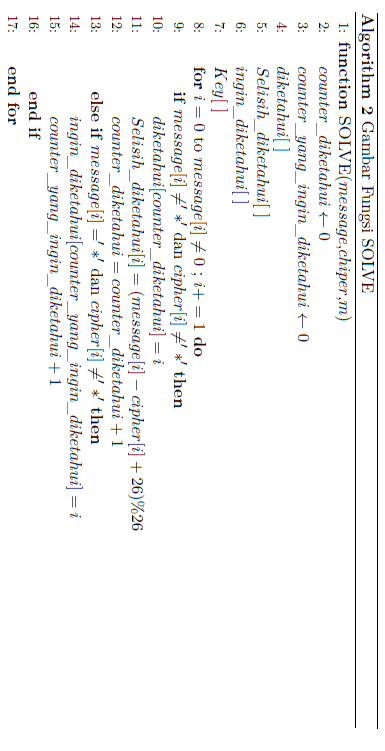
\includegraphics[scale=0.43]{images/bab3/solvefx1.png}
		\caption{Gambar Fungsi SOLVE (1)}
		\label{fig:solvefx1}
	\end{figure}
	\begin{figure}[H]
		\centering
		\resizebox{\textwidth}{!}{%
		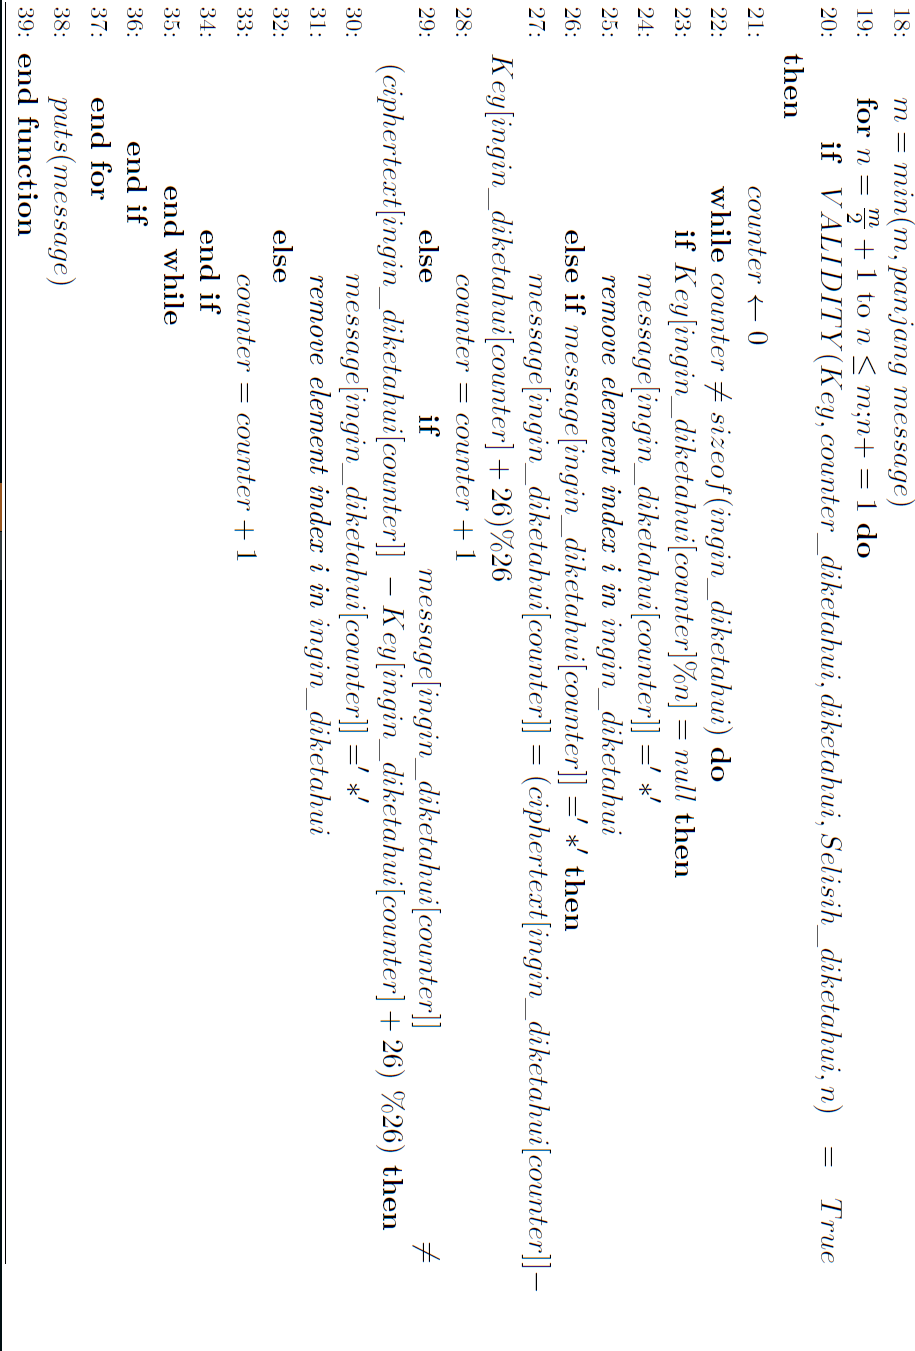
\includegraphics[scale=0.4]{images/bab3/solvefx21.png}}
		\caption{Gambar Fungsi SOLVE (2)}
		\label{fig:solvefx2}
	\end{figure}
	
	\begin{table}[H]
	 	\caption{Penjelasan variabel yang digunakan dalam fungsi SOLVE}
		%\resizebox{\textwidth}{!}{%
		\begin{tabular}   {|p{3cm}|p{6cm}|}\hline
		Nama Variabel&Penjelasan \\ \hline
		m&Digunakan untuk menerima dan menyimpan masukan batas atas panjang kunci dari fungsi MAIN. \\ \hline
		message&Digunakan untuk menerima dan menyimpan masukan \plaintext dari fungsi MAIN.\\ \hline
		cipher&Digunakan untuk menerima dan menyimpan masukan \ciphertext dari fungsi MAIN. \\ \hline
		counter\verb|_|diketahui&Digunakan untuk menghitung indeks jumlah \plaintext dan \ciphertext yang tidak "*". \\ \hline
		counter\verb|_|yang\verb|_| ingin\verb|_|diketahui&Digunakan untuk menghitung jumlah indeks \ciphertext tidak bernilai "*" dan \plaintext bernilai "*". \\ \hline
		diketahui&Merupakan suatu \textit{array} yang digunakan untuk menyimpan indeks di mana \plaintext dan \ciphertext yang tidak "*". \\ \hline
		Selisih\verb|_|diketahui&Merupakan suatu \textit{array} yang digunakan untuk menyimpan selisih antara \plaintext dan \ciphertext di mana \plaintext dan \ciphertext pada indeks tersebut tidak bernilai "*". \\ \hline
		ingin\verb|_|diketahui&Merupakan suatu \textit{array} yang digunakan untuk menyimpan indeks di mana  \ciphertext tidak bernilai "*" dan \plaintext bernilai "*" pada indeks tersebut. \\ \hline
		\end{tabular}%}
		\label{tab:solvar}
	\end{table}
  	\begin{table}[H]
	 	
		%\resizebox{\textwidth}{!}{%
		\begin{tabular}   {|p{3cm}|p{6cm}|}\hline
		%Nama Variabel&Penjelasan \\ \hline
		
		
		Key&Merupakan suatu \textit{array} yang digunakan untuk menyimpan hasil yang diperoleh dari fungsi VALIDITY \\ \hline
		\end{tabular}%}
		\label{tab:solvar}
	\end{table}	
	
	
	\subsection{Desain Fungsi VALIDITY}
	Fungsi ini digunakan untuk memvalidasi suatu panjang kunci yang sekarang dicek kebenarannya. Gambar mengenai fungsi VALIDITY dapat dilihat pada gambar \ref{fig:validity}. Penjelasan mengenai fungsi ini terdapat pada subbab \ref{chapter:solving}. %Masukan pada fungsi ini berupa Key, counter\verb|_|diketahui, diketahui, Selisih\verb|_|diketahui, n. Keluaran dari fungsi ini berupa Key, dan nilai benar atau salah. Proses yang dilakukan pada fungsi ini adalah mencari apakah suatu panjang kunci dapat digunakan atau tidak atau merupakan bagian dari modifikasi dari algoritma \textit{Kasiski Examination}. 
	
		\begin{table}[H]
	 	\caption{Masukan, Proses, dan Keluaran fungsi MAIN}
		%\resizebox{\textwidth}{!}
		\label{tab:iomain}
	\end{table}
	
 \begin{figure}[H]
		\centering
		\resizebox{\textwidth}{!}{%
		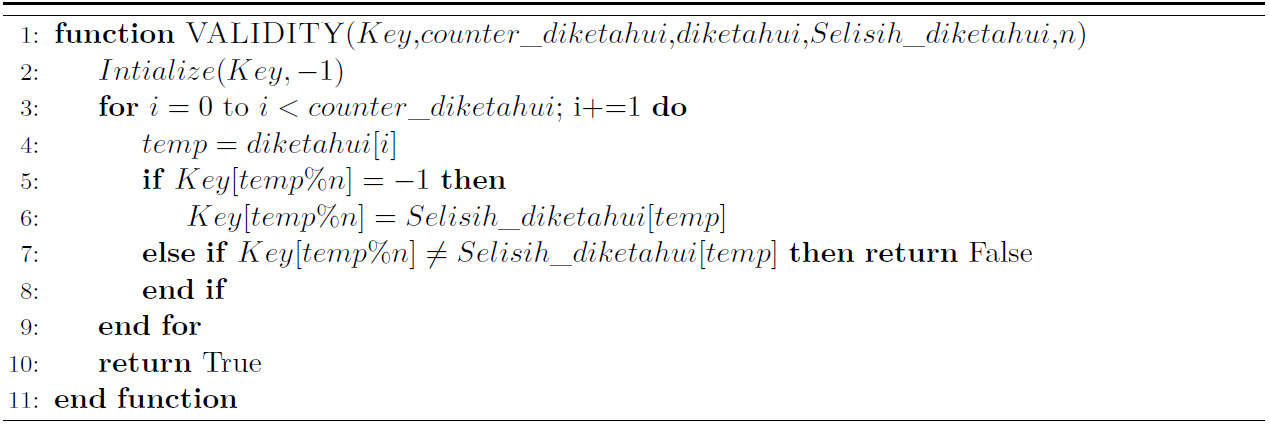
\includegraphics[scale=0.5]{images/bab3/validity.png}}
		\caption{Gambar Fungsi VALIDITY}
		\label{fig:validity}
	\end{figure}
	
	 \begin{table}[H]
	 	\caption{Penjelasan variabel yang digunakan dalam fungsi VALIDITY}
		%\resizebox{\textwidth}{!}{%
		\begin{tabular}   {|p{3cm}|p{6cm}|}\hline
		Nama Variabel&Penjelasan \\ \hline
		Key&Merupakan suatu \textit{array} yang digunakan untuk menyimpan blok kunci yang telah dibentuk. \\ \hline
		counter\verb|_|diketahui&Digunakan untuk menerima dan menyimpan masukan counter\verb|_|diketahui dari fungsi SOLVE.\\ \hline
		diketahui&Merupakan suatu \textit{array} yang digunakan untuk menerima dan menyimpan masukan variabel diketahui pada fungsi SOLVE. \\ \hline
		Selisih\verb|_|diketahui&Merupakan suatu \textit{array} yang digunakan untuk menerima dan menyimpan Selisih\verb|_|diketahui dari fungsi SOLVE. \\ \hline
		n&Digunakan untuk menerima dan menyimpan posisi iterasi saat ini dari fungsi SOLVE. \\ \hline
		\end{tabular}%}
		\label{tab:solvar}
	\end{table}